\documentclass[10pt,twocolumn,letterpaper]{article}
\usepackage[margin=0.9in,columnsep=0.28in]{geometry}
\usepackage[T1]{fontenc}
\usepackage[utf8]{inputenc}
\usepackage{times}
\usepackage{amsmath,amssymb}
\usepackage{graphicx}
\usepackage{booktabs}
\usepackage{array,multirow}
\usepackage{xcolor,colortbl}
\usepackage{caption}
\usepackage[colorlinks=true,allcolors=blue,breaklinks=true]{hyperref}
\captionsetup{font=small,labelfont=bf}
\graphicspath{{figures/}}
\pagestyle{plain}
\title{\textbf{Not All Organs Break Equally: Per-Organ Fragility of Abdominal MRI Segmentation under k-Space Acceleration}}
\author{Alfin William Adi Putra\\ \texttt{alfinwilliam30@gmail.com}}
\date{August 2026 --- preprint}
\begin{document}
\maketitle

\begin{abstract}
Accelerated MRI is certified with image-quality metrics, but its output increasingly feeds a downstream segmentation network rather than a radiologist's eye. Under retrospective k-space undersampling of multi-organ abdominal MRI, we show that segmentation does not degrade uniformly: from $R{=}1$ to $R{=}8$, per-organ Dice loss spans an order of magnitude (adrenal $-0.198$ vs.\ liver $-0.019$; 13/13 organs Holm-significant; replicated on a second dataset). This fragility is predictable from anatomy alone: an organ's spectral centroid --- the energy-weighted mean radial frequency of its k-space content --- rank-predicts its drop (Spearman $0.863/0.855$; five-fold CV $0.841\pm0.023$) and survives control for organ volume (partial $\rho{=}0.75$). The link is mechanistic: on real multicoil knee k-space, the energy an undersampling mask removes rank-predicts the Dice degradation ($0.952$ pooled; $0.94$ within fixed $R$). We translate the law into a released per-organ acceleration budget that agrees across datasets ($\rho{=}0.989$). Extending the known aggregate decoupling of reconstruction metrics from task performance, we show the blindness persists at per-organ resolution: within a fixed acceleration ($R\geq4$), SSIM and PSNR carry essentially no information about per-organ failure (at $R{=}8$, $\rho{=}-0.093/-0.205$ vs.\ tail-organ Dice). Mixed-acceleration training is the one intervention that helps, and it helps the worst organs most (gain vs.\ baseline Dice Spearman $\rho{=}-0.93$); fragility-guided reconstruction ties it, while fragility-weighted losses and fragility-steered learned sampling fail: at a fixed acquisition and scale, per-organ fragility is not fixable by post-hoc modeling. Code, budgets, and the predictor are released.
\end{abstract}

\section{Introduction}
\label{sec:intro}

Accelerated MRI shortens scan time by sampling only a fraction of k-space --- the Fourier domain of the image --- and reconstructing the remainder \cite{lustig2007,hammernik2018,sriram2020}. The quality of that reconstruction is almost universally certified with image-fidelity metrics such as PSNR and SSIM \cite{zbontar2018fastmri,muckley2021}. Yet in a growing number of clinical and research pipelines the image is never read by a human: it is consumed by a downstream network, most often a segmentation model. The certificate and the consumer can disagree sharply. At eightfold acceleration ($R{=}8$), an abdominal reconstruction still scores SSIM $0.82$ --- by the standard report card, a usable image --- while the Dice score of the adrenal glands has dropped by $0.198$ and that of the liver by only $0.019$ (Fig.~\ref{fig:money}). Recent benchmarks established the aggregate form of this decoupling: reconstruction fidelity and downstream segmentation accuracy come apart \cite{morshuis2025,tolpadi2023,muckley2021}. But those studies report a single Dice number averaged over anatomy, on knee data, and stop at the fact \emph{that} the decoupling exists. They do not ask \emph{which} structures fail, by \emph{how much}, or \emph{why} --- and it is precisely that per-structure picture that determines whether an accelerated protocol is safe for a given clinical target.

\begin{figure*}[t]
  \centering
  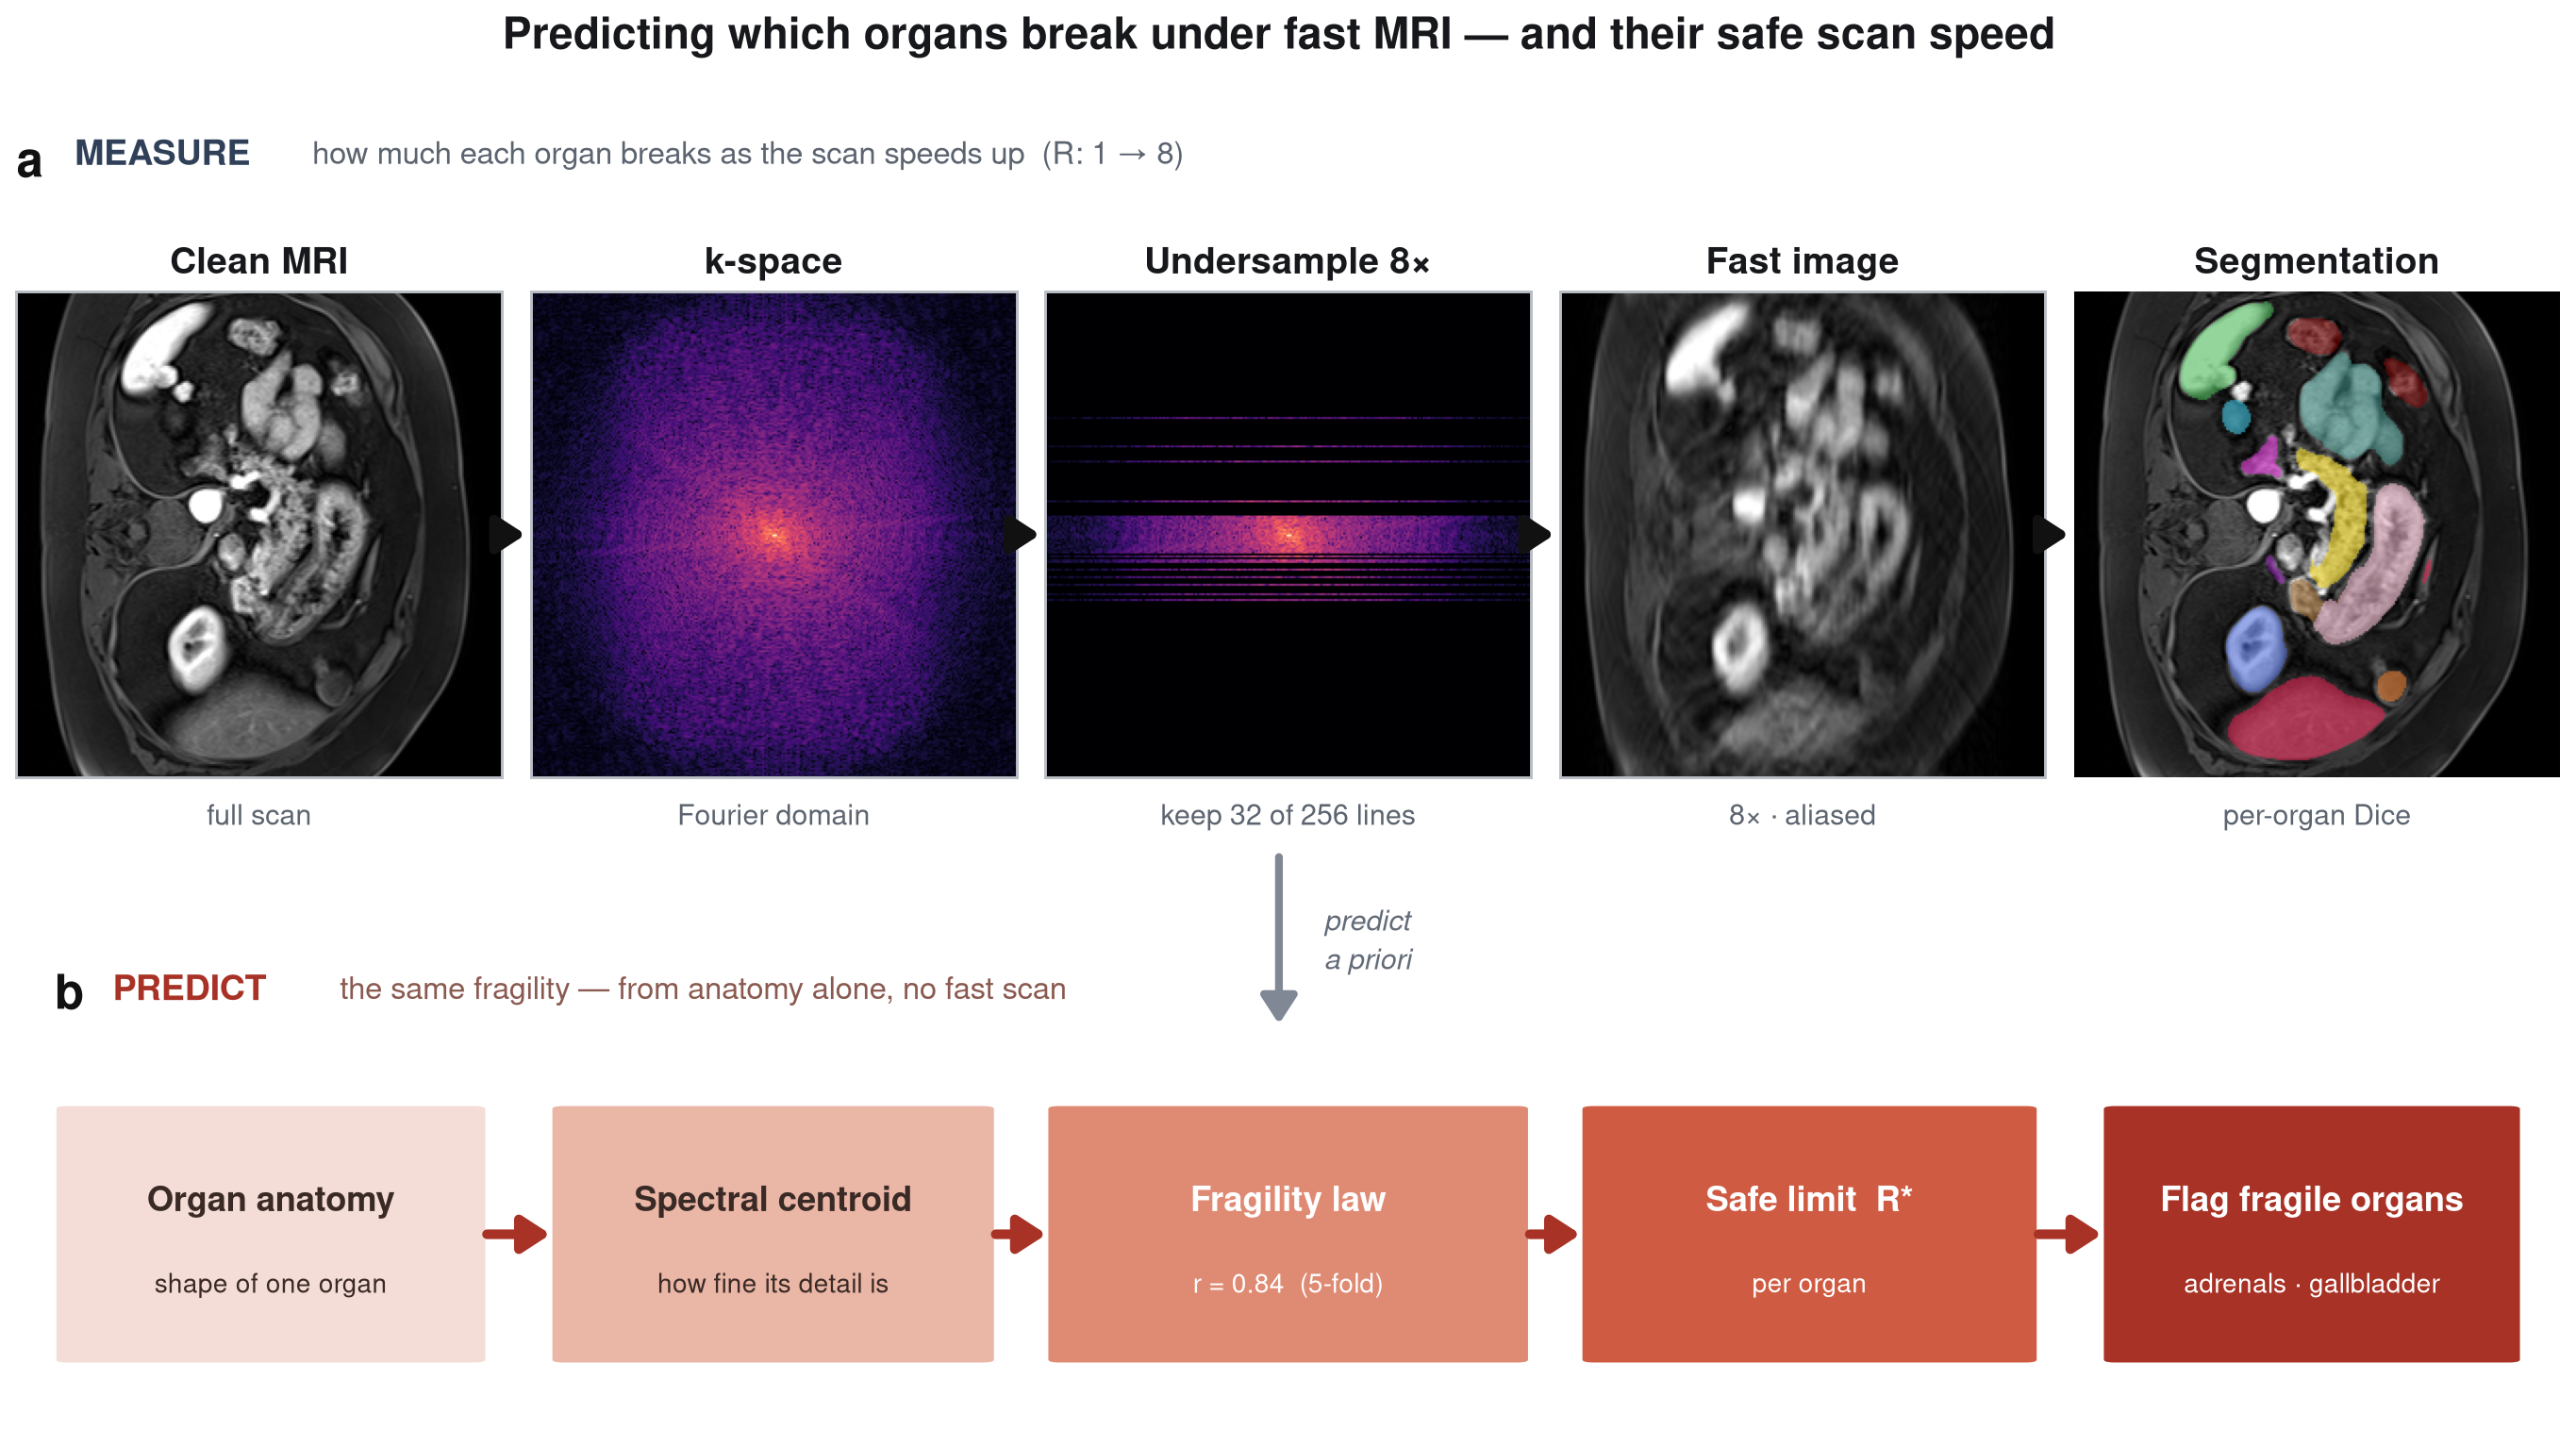
\includegraphics[width=\linewidth]{figure1.png}
  \caption{\textbf{The image looks fine; the task quietly fails --- and not all organs fail equally.}
  Left: at $R{=}8$ the reconstruction retains SSIM $0.82$, a score that would pass a conventional image-quality check, while adrenal segmentation has lost $0.198$ Dice and the liver only $0.019$.
  Right: per-organ fan-out of Dice under increasing acceleration --- the degradation spans a $10.2\times$ range across the thirteen abdominal organs (all Holm-significant; ordering replicated on a second dataset). Both the aggregate Dice and the image metric hide this per-organ structure, which is the object of this paper.}
  \label{fig:money}
\end{figure*}

We take up that question in multi-organ abdominal MRI and find that failure under acceleration is strikingly non-uniform. Under retrospective variable-density undersampling with an nnU-Net segmenter \cite{isensee2021}, per-organ Dice loss from $R{=}1$ to $R{=}8$ spans an order of magnitude --- a $10.2\times$ spread from the adrenal glands ($-0.198$) to the liver ($-0.019$) --- with all thirteen organs significant after Holm correction on MRISegmentator \cite{mrisegmentator2024} and the ordering replicated on AMOS-MRI \cite{amos2022}. A single averaged number hides this entirely. More importantly, the ordering is predictable \emph{from anatomy alone}. Define an organ's spectral centroid as the energy-weighted mean radial frequency of its k-space content,
\begin{equation}
  c_\Omega \;=\; \frac{\sum_{k} \lVert k \rVert \,\bigl|\hat{x}_\Omega(k)\bigr|^{2}}{\sum_{k} \bigl|\hat{x}_\Omega(k)\bigr|^{2}},
  \label{eq:centroid}
\end{equation}
where $\hat{x}_\Omega$ is the Fourier transform of the organ-windowed image --- computable from the fully sampled image before any accelerated acquisition or segmenter is run. This single number rank-predicts the organ's Dice drop with Spearman $0.863$ on MRISegmentator and $0.855$ on AMOS (five-fold cross-validated $0.841\pm0.023$), and it survives control for organ volume across a $421\times$ size range (partial $\rho{=}0.750$, $p{=}0.005$) while the reverse partial dies ($p{=}0.58$): the law is not a restatement of ``small organs are hard.'' Two scope notes keep the claim honest. First, on AMOS a high-frequency image-energy descriptor ties the centroid exactly ($\rho{=}0.855$ for both), so we claim a \emph{high-frequency anatomy signature} with the centroid as its physical representative; the centroid leads only on MRISegmentator ($0.863$ vs.\ $0.852$ next best). Second, on the thirteen abdominal organs the centroid is confounded with baseline difficulty (partial $\rho{=}0.16$, n.s.); the two dissociate on 41 whole-body TotalSegmentator structures \cite{wasserthal2023totalseg}, where the centroid predicts the drop over and above baseline difficulty at full resolution (partial $\rho{=}0.389$, permutation $p{=}0.0067$; $\rho{=}0.66$, $p{=}0.0001$ on the 30 gradually degrading structures; $72.6\%$ of 296 difficulty-matched pairs order correctly) --- though under a fast-reconstruction preprocessing the partial attenuates to non-significance ($0.141$), so the dissociation is claimed for full resolution only. The predictor is grounded in mechanism rather than curve fitting: on real multicoil knee k-space \cite{desai2022skmtea}, the fraction of spectral energy that the undersampling mask removes rank-predicts the Dice degradation at Spearman $0.952$ pooled --- and still $0.94$ at fixed $R\in\{6,8\}$, where the shared acceleration trend cannot explain it --- escaping the Parseval tautology that removed energy merely equals image error ($r{=}0.978$). Our abdominal k-space is simulated; as a fidelity check, a full complex multicoil forward model ($A = M F S$) preserves the per-organ ordering of the magnitude-only pipeline at Spearman $0.978$.

This predictability has a practical payoff and a sobering flip side. On the payoff side, we convert the law into a per-organ \emph{acceleration budget} $R^{*}$ --- the highest acceleration at which an organ's Dice loss stays within tolerance --- computable a priori and consistent across datasets (ordering $\rho{=}0.989$): the adrenal glands are unsafe beyond $R{\approx}4$ while the liver and kidneys tolerate $R{=}8$ and beyond. On the flip side, the metric that certifies accelerated protocols is blind at exactly this resolution: within a fixed acceleration ($R\geq4$), SSIM carries essentially no information about per-organ segmentation success, and at $R{=}8$ neither SSIM nor PSNR predicts tail-organ Dice across cases ($\rho{=}-0.093$ and $-0.205$). Finally, we ask what actually helps the fragile organs. The one intervention that does is matching the training distribution to the degradation: mixed-acceleration training improves tail-organ Dice on 239 of 240 abdominal cases ($p{=}4\times10^{-41}$; $+0.134$ on real knee k-space), with an honestly reported magnitude of $+0.088$ against a fixed-$R$ model deployed out of distribution and $+0.019$ against a matched baseline --- and its mechanism is weakest-organ regularization: it helps the worst organs most (per-organ gain vs.\ baseline Dice Spearman $\rho{=}-0.93$). Everything else we tried is a documented tie or negative: fragility-guided reconstruction ties mixed-$R$ ($p{=}0.18$); a fragility-weighted segmentation loss is indistinguishable from uniform weighting ($p{=}0.77$); a per-organ weighting sweep stays within seed noise; and in a 2D learned-sampling proof of concept \cite{bahadir2020loupe}, learned masks beat fixed variable-density sampling ($+0.044\pm0.025$ across seeds; seed-level $p{=}0.128$, underpowered at $n{=}3$) but adding a fragility prior is a wash ($-0.007\pm0.004$) and a fragility-steered variant is negative ($-0.089$). The through-line: per-organ fragility is unfixable by post-hoc modeling at a fixed acquisition and scale --- only changing what is acquired, or training on the degradation itself, moves it. Throughout, we are explicit about the inferential unit: the organ-level analyses rest on $n{=}13$ (MRISegmentator) and $n{=}11$ (AMOS) shared organ identities, and the case-clustered bootstrap CI on the law ($[0.824, 0.879]$ over 240 cases) addresses case-sampling noise only, not the small organ count.

\paragraph{Contributions.}
\begin{enumerate}
  \item \textbf{The first per-organ characterization} of segmentation fragility under k-space acceleration in multi-organ abdominal MRI (prior work is aggregate-Dice, knee-only \cite{morshuis2025,tolpadi2023}): a $10.2\times$ spread, 13/13 organs Holm-significant, replicated across two datasets.
  \item \textbf{A spectral predictor} computable from anatomy alone --- a high-frequency signature with the centroid as its representative --- that forecasts fragility beyond organ size (partial $\rho{=}0.750$ over log-volume) and, on 41 whole-body structures at full resolution, dissociates from baseline difficulty (partial $\rho{=}0.389$, $p{=}0.0067$).
  \item \textbf{A real-k-space mechanism}: the spectral energy removed by undersampling predicts the downstream task drop (Spearman $0.952$ pooled, $0.94$ within fixed $R$) --- a non-tautological energy$\rightarrow$task link beyond the Parseval identity.
  \item \textbf{A released per-organ acceleration budget}, cross-dataset consistent (ordering $\rho{=}0.989$) and usable a priori for protocol selection.
  \item \textbf{An evaluation-validity result at per-organ resolution}: within a fixed acceleration ($R\geq4$), image-quality metrics are blind to per-organ task failure (at $R{=}8$: SSIM $\rho{=}-0.093$, PSNR $\rho{=}-0.205$ vs.\ tail-organ Dice), extending the aggregate recon--task decoupling of \cite{morshuis2025,tolpadi2023} to the resolution that matters clinically.
  \item \textbf{A prescription with honest negatives}: mixed-$R$ training helps the worst organs most (gain vs.\ baseline Dice Spearman $\rho{=}-0.93$), while fragility-guided reconstruction ties it ($p{=}0.18$), fragility-weighted losses match uniform, and fragility-steered learned sampling fails --- per-organ fragility is unfixable by post-hoc modeling at a fixed acquisition and scale.
\end{enumerate}

\section{Related work}
\label{sec:related}

\paragraph{Accelerated MRI and its evaluation.}
Sub-Nyquist acquisition with compressed-sensing~\cite{lustig2007} or learned reconstruction~\cite{hammernik2018,sriram2020,akcakaya2022,heckel2024} is now standard practice, and the public benchmarks that drove this progress score it almost exclusively with image-fidelity metrics~\cite{zbontar2018fastmri,knoll2020}. The limits of that yardstick are documented: the fastMRI challenge reported that PSNR/SSIM rankings fail to penalize hallucinated or missing pathology~\cite{muckley2021}, and clinical validation of accelerated protocols still rests on reader studies rather than metrics~\cite{radmanesh2022,chaudhari2020}.

\paragraph{Reconstruction--task decoupling.}
When the consumer of the image is a downstream model rather than a radiologist, reconstruction fidelity and task performance decouple. In the K2S challenge, the best segmentation at $8\times$ acceleration came from a pipeline with among the worst reconstruction metrics~\cite{tolpadi2023}; SKM-TEA pairs raw k-space with downstream tasks to make exactly this measurable~\cite{desai2022skmtea}; and Morshuis et al.\ show on knee MRI that reconstruction metrics do not predict segmentation utility~\cite{morshuis2025}. We credit these results as prior work: the \emph{aggregate} decoupling of reconstruction metrics from task performance is established. What they leave open --- reporting a single Dice averaged over anatomy, on knee data --- is \emph{which} structures fail, by how much, and why; our contribution is the per-organ resolution of the same question (our within-$R$ analysis is scoped to $R\ge 4$). Segmentation directly under undersampling has otherwise been studied for single structures, e.g.\ breast lesions~\cite{rotkopf2026}, not for multi-organ anatomy.

\paragraph{Spectral bias and frequency robustness.}
Deep networks fit low frequencies first~\cite{rahaman2019,xu2019}, and model robustness has a characteristic Fourier signature~\cite{yin2019}. Those are statements about the \emph{network's} spectrum. Our fragility law is a statement about the \emph{anatomy's}: variable-density undersampling deletes high radial frequencies, so organs whose discriminative content lives there are hit hardest, whatever the model's bias.

\paragraph{Per-organ difficulty.}
Multi-organ benchmarks report stable per-organ difficulty orderings on fully sampled images --- TotalSegmentator~\cite{wasserthal2023totalseg}, MRISegmentator~\cite{mrisegmentator2024}, AMOS~\cite{amos2022} --- commonly summarized as ``small organs are hard''~\cite{isensee2021}. That describes difficulty at a \emph{fixed} acquisition. We characterize its sensitivity \emph{to} the acquisition: which organs lose Dice as $R$ rises. The two are not the same --- below, large hollow organs break while a small compact one holds up.

\paragraph{Sampling and training-distribution design.}
A rich line of work learns or optimizes the sampling pattern itself~\cite{bahadir2020loupe,huijben2020,weiss2021,sanchez2020,defazio2020}, sequentially or by policy~\cite{bakker2020,pineda2020}, and for segmentation specifically~\cite{razumov2023}; training across acceleration factors has been used to make \emph{reconstruction} robust to the rate~\cite{yao2022}. We use this machinery as instruments, not contributions: learned masks and mixed-$R$ training are evaluated \emph{per organ}, including as honest negatives.

In sum, prior work establishes that aggregate reconstruction metrics decouple from an aggregate task score, on knee data. We add the layer beneath the aggregate: which organs break under acceleration, at what rate they break (a released per-organ budget $R^{*}$), why (a frequency-content account with a real-k-space energy mechanism), and what does --- and does not --- fix it.

\section{Per-organ fragility under acceleration}
\label{sec:fragility}

\subsection{Setup}
\paragraph{Datasets.}
Our primary dataset is MRISegmentator-Abdomen~\cite{mrisegmentator2024}: 195 patients with four T1 phases each, split at the \emph{patient} level 135/60 into 540 training and 240 test series. We analyze the 13 major abdominal organs listed in Table~\ref{tab:fragility}. The MRI subset of AMOS22~\cite{amos2022} serves as the replication dataset on the 11 organ identities it shares with MRISegmentator (AMOS lacks colon and small-bowel labels).

\paragraph{Retrospective undersampling.}
We apply variable-density Cartesian undersampling with a fully sampled autocalibration center to the full-FOV k-space of each series, at $R\in\{1,2,4,6,8\}$ ($R{=}1$ is the fully sampled baseline). For each case, masks are drawn with a generator seeded by a hash of the case identifier, so the degradation varies realistically across cases yet is deterministic and reproducible. Undersampling is simulated from magnitude images, as no public abdominal raw-k-space dataset with multi-organ labels exists; a control with a full complex multicoil forward operator ($A = M F S$) preserves the per-organ ordering (Spearman 0.978). Ground truth is always the annotation of the fully sampled series --- only the network's input is degraded.

\paragraph{Model and statistics.}
The segmenter is nnU-Net~v2, 3D full-resolution~\cite{isensee2021}, trained once at $R{=}2$ and deployed at every $R$ --- the practical setting of a fixed model meeting varying acceleration --- with no test-time augmentation. Per organ we report case-mean Dice, NSD, and HD95 over the 240 test series; the $R{=}1{\to}8$ Dice drop is tested with a paired Wilcoxon signed-rank test over cases, Holm-corrected across the 13 organs, with a paired Cohen's~$d$ as effect size.

\subsection{An order-of-magnitude spread}

\begin{table}[t]
\centering
\caption{Per-organ fragility on MRISegmentator ($n{=}240$ test series), sorted by Dice drop from $R{=}1$ to $R{=}8$. All 13 drops are individually significant (paired Wilcoxon, all $p<10^{-31}$, surviving Holm correction). $^\dagger$:~small-volume (``tail'') organs.}
\label{tab:fragility}
\small
\begin{tabular}{lcccc}
\toprule
Organ & Dice $R{=}1$ & Dice $R{=}8$ & $\Delta$Dice & Cohen's $d$ \\
\midrule
adrenal L$^\dagger$   & 0.638 & 0.440 & $-0.198$ & 1.21 \\
adrenal R$^\dagger$   & 0.645 & 0.459 & $-0.186$ & 1.20 \\
gallbladder$^\dagger$ & 0.895 & 0.725 & $-0.170$ & 1.19 \\
colon                 & 0.932 & 0.769 & $-0.163$ & 2.24 \\
duodenum$^\dagger$    & 0.858 & 0.717 & $-0.141$ & 1.86 \\
esophagus$^\dagger$   & 0.869 & 0.741 & $-0.128$ & 1.30 \\
small bowel           & 0.940 & 0.826 & $-0.113$ & 2.42 \\
pancreas$^\dagger$    & 0.908 & 0.835 & $-0.073$ & 1.75 \\
stomach               & 0.947 & 0.881 & $-0.066$ & 1.14 \\
spleen                & 0.969 & 0.921 & $-0.047$ & 0.61 \\
kidney L              & 0.969 & 0.929 & $-0.040$ & 0.83 \\
kidney R              & 0.974 & 0.935 & $-0.039$ & 1.15 \\
liver                 & 0.989 & 0.970 & $-0.019$ & 1.24 \\
\bottomrule
\end{tabular}
\end{table}

\begin{figure*}[t]
\centering
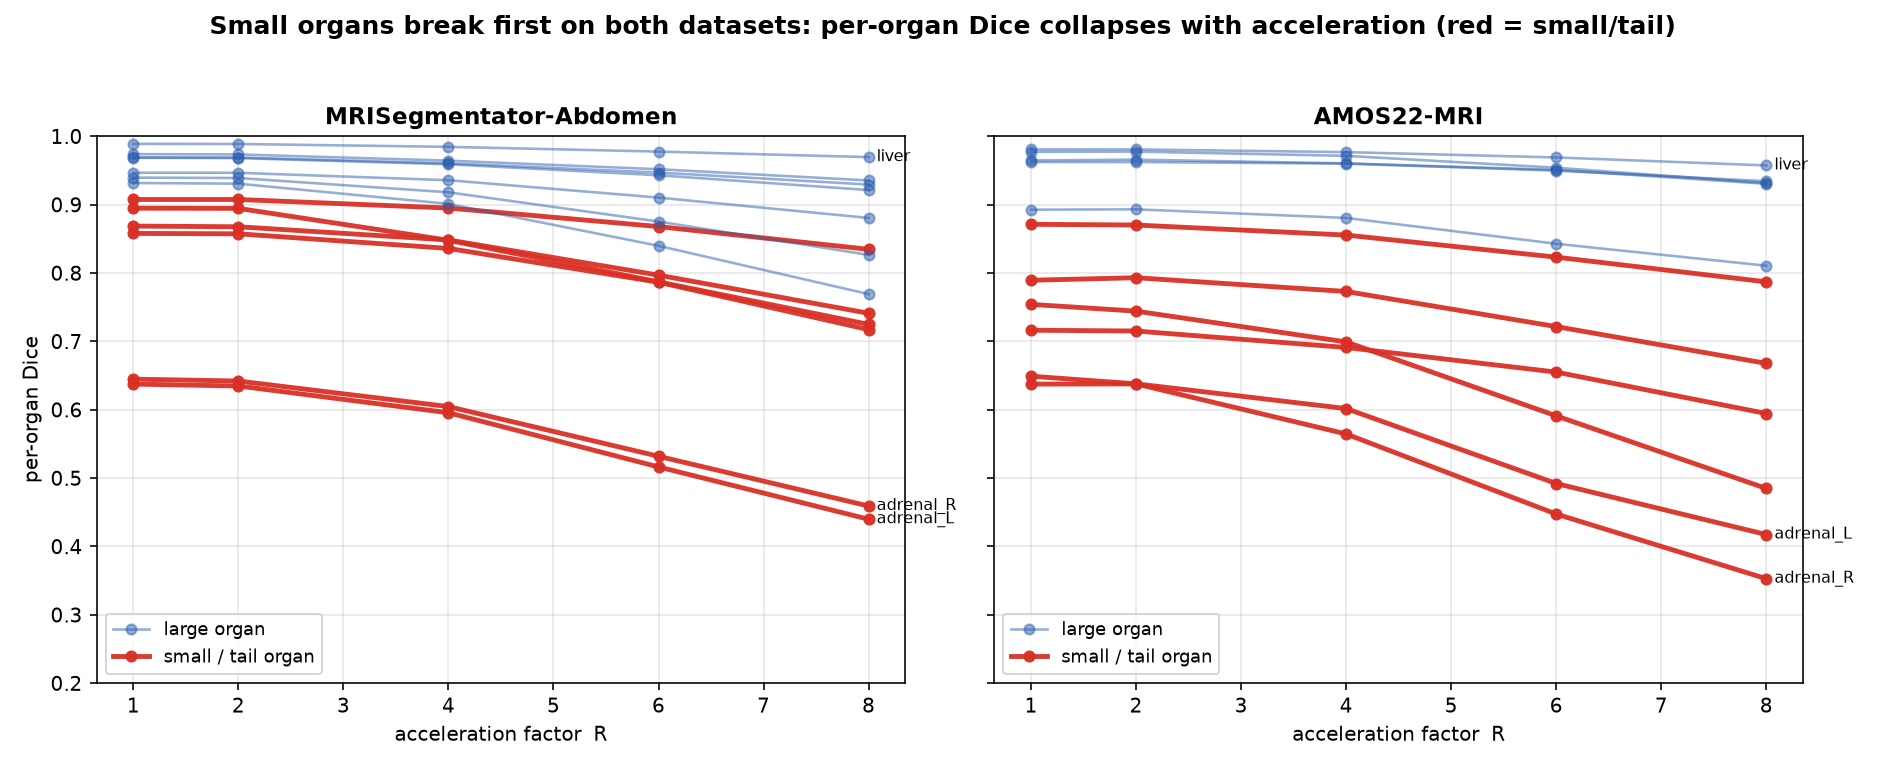
\includegraphics[width=\linewidth]{fragility_combined.png}
\caption{Per-organ Dice versus acceleration $R$ on MRISegmentator and AMOS22-MRI. Degradation is negligible at $R{=}2$ and fans out from $R{=}4$ onward: the fragile organs (adrenals, gallbladder, duodenum, esophagus, colon) separate from the robust compact organs (liver, kidneys, spleen). The same fan-out appears on both datasets over the 11 shared organ identities.}
\label{fig:fragilitycurves}
\end{figure*}

Degradation under acceleration is strikingly non-uniform (Table~\ref{tab:fragility}, Fig.~\ref{fig:fragilitycurves}). From $R{=}1$ to $R{=}8$ the left adrenal loses 0.198 Dice while the liver loses 0.019 --- a $10.2\times$ spread --- with every organ in between falling into a stable ordering. All thirteen drops are individually significant (paired Wilcoxon over 240 cases, all $p<10^{-31}$, trivially surviving Holm correction), with paired effect sizes $d$ from 0.61 to 2.42. The damage is invisible at $R{=}2$ --- every organ sits within 0.003 Dice of its fully sampled value --- and concentrates at $R\ge 4$, steepening through $R{=}8$. Boundary metrics tell the same story: over the same sweep, colon HD95 grows from 12.5 to 40.5\,mm and left-adrenal NSD falls from 0.65 to 0.44.

Grouped, the six small-volume ``tail'' organs ($\dagger$ in Table~\ref{tab:fragility}) lose a mean $-0.149$ Dice versus $-0.070$ for the seven remaining organs (five-fold: $0.150$ vs.\ $0.071$) (a $2.1\times$ contrast, stable across five training folds; the case-level group difference is large, $d{=}1.48$, $p{=}3.1\times10^{-26}$). The same fan-out replicates on AMOS22-MRI over the shared organ identities (Fig.~\ref{fig:fragilitycurves}), so the ordering is not an artifact of one dataset or one annotation protocol.

An honest nuance: fragility is \emph{not} a pure size ordering. The colon ($-0.163$) and small bowel ($-0.113$) are among the largest structures yet break early --- they are thin-walled and hollow --- while the pancreas ($-0.073$), nominally a small tail organ, is compact and solid and holds up better than either. The most robust organs are uniformly the compact solid ones (liver, kidneys, spleen). At this descriptive level the defensible characterization is a disjunction: fragile organs have \emph{small volume or a thin, hollow boundary}. This is also why the $2.1\times$ group contrast understates the $10.2\times$ adrenal--liver contrast: the pancreas dilutes the tail mean while the colon inflates the robust one. That an apparent disjunction should have a single explanation is the subject of the next section --- both small structures and thin, convoluted boundaries concentrate their k-space energy at high radial frequency, which is precisely what variable-density undersampling deletes first.

\section{A spectral law predicts who breaks}
\label{sec:law}

The per-organ ordering of fragility is not arbitrary: it is predictable \emph{from anatomy alone}, before any accelerated acquisition is simulated or any segmenter is run. For an organ occupying image region $\Omega$, let $x_\Omega = \mathbb{1}_\Omega \odot x$ denote the organ-windowed fully sampled image and $\hat{x}_\Omega$ its discrete Fourier transform. We define the organ's \emph{spectral centroid} as the energy-weighted mean radial spatial frequency of its k-space content,
\begin{equation}
c_\Omega \;=\; \frac{\displaystyle\sum_{\mathbf{k}} \lVert \mathbf{k} \rVert \,\bigl|\hat{x}_\Omega(\mathbf{k})\bigr|^{2}}{\displaystyle\sum_{\mathbf{k}} \bigl|\hat{x}_\Omega(\mathbf{k})\bigr|^{2}},
\label{eq:centroidlaw}
\end{equation}
computable from one fully sampled scan and the organ mask, with no reconstruction and no segmentation model in the loop.

\begin{figure}[t]
\centering
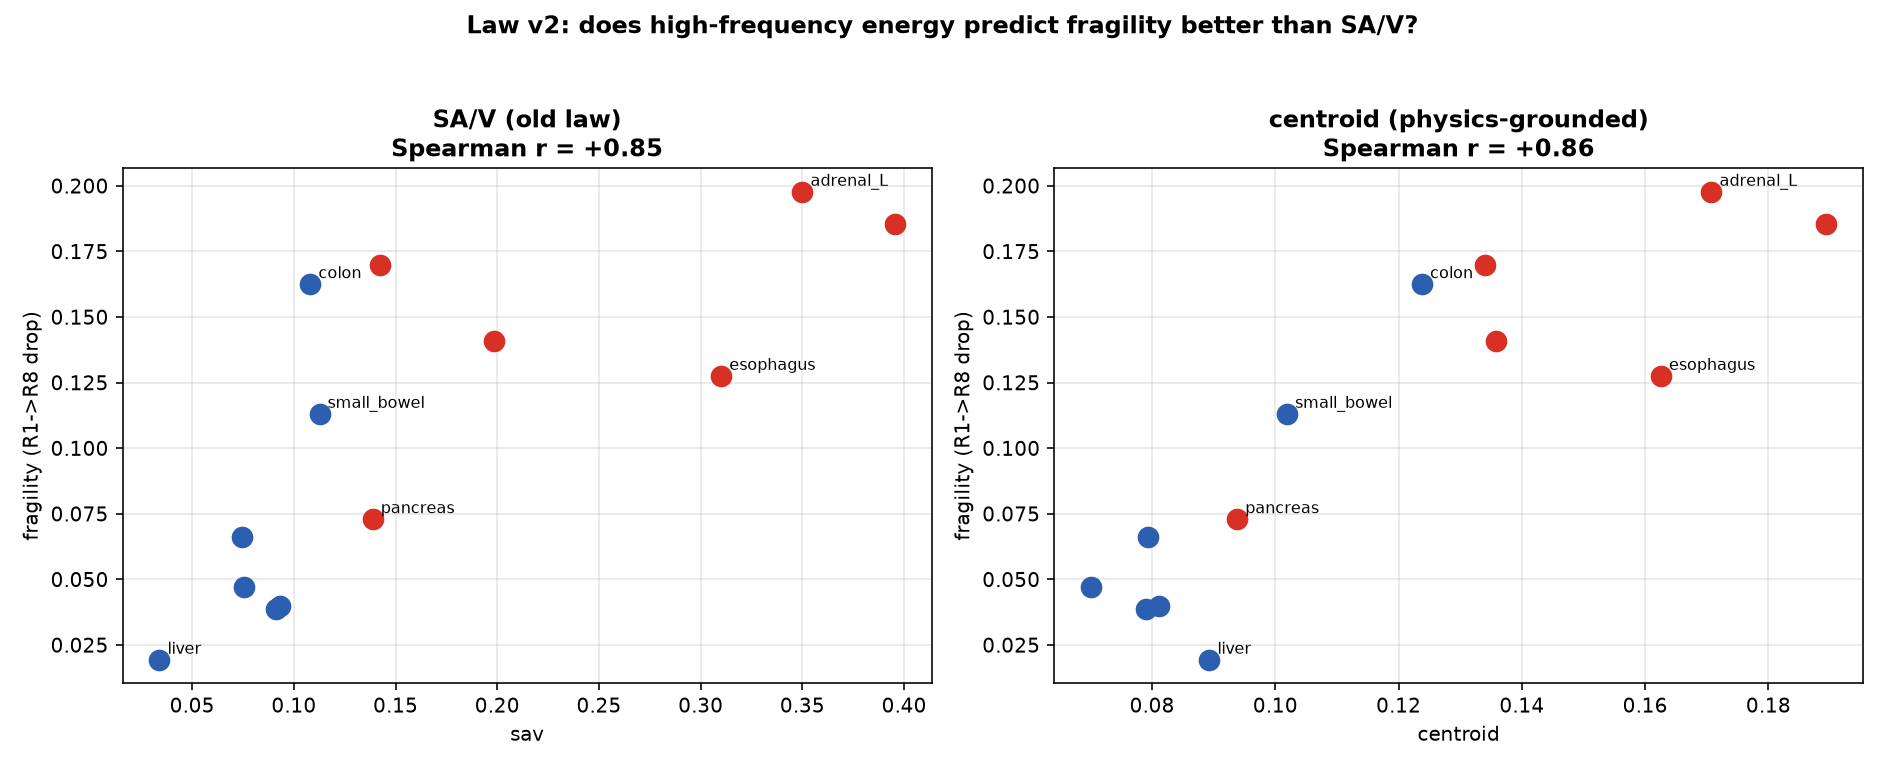
\includegraphics[width=\linewidth]{m0_law_v2.png}
\caption{\textbf{The spectral law.} Per-organ Dice drop ($R{=}1{\to}8$) against the a-priori spectral centroid $c_\Omega$ on MRISegmentator (Spearman $\rho=0.863$; AMOS: $0.855$). Organs whose discriminative content sits at high radial frequency (adrenals, gallbladder) are exactly the ones acceleration deletes first; low-centroid compact organs (liver, kidneys) survive.}
\label{fig:law}
\end{figure}

\paragraph{The prediction.}
This single number rank-predicts an organ's Dice drop at $R{=}8$ with Spearman $\rho=0.863$ on MRISegmentator \cite{mrisegmentator2024} and $0.855$ on AMOS-MRI \cite{amos2022} (Fig.~\ref{fig:law}). The relation is stable under resampling: five-fold cross-validation gives $\rho = 0.841 \pm 0.023$, and a selection-corrected permutation test against four rival descriptors gives $p=0.0015$ (MRISeg) and $0.0053$ (AMOS). In pure rank terms the strongest geometric rival, surface-area-to-volume ratio, nearly ties in fold-CV ($0.830 \pm 0.023$), but calibrated prediction separates them: leave-one-organ-out cross-validated $R^2$ is $0.70/0.60$ (MRISeg/AMOS) for the centroid against $0.45/0.46$ for SA:V. A case-clustered bootstrap (resampling the 240 test cases, not the organs) puts the law at $\rho=0.863$, 95\% CI $[0.824, 0.879]$ --- but we are explicit about what this interval covers: it addresses case-sampling noise \emph{only}. The inferential unit for the law itself remains the organ, and there are only 13 organs on MRISegmentator and 11 shared identities on AMOS; no bootstrap over cases enlarges that $n$. We state this limitation plainly rather than dressing the law in a CI it has not earned at the organ level.

\paragraph{Not just small organs.}
The sharpest cheap objection is that the centroid is a proxy for size. It is not: controlling for log-volume across a $421\times$ size range leaves the centroid effect intact (partial $\rho = +0.750$, $p=0.005$), whereas the reverse partial --- volume given centroid --- dies ($p=0.58$). Size predicts fragility only through its correlation with spectral content, not the other way around.

\paragraph{Not just baseline difficulty.}
A subtler objection is that high-centroid organs are simply the hard ones, so the law restates clean-image difficulty. On the 13 abdominal organs this cannot be settled: centroid and clean Dice are entangled ($r=-0.93$), and the partial correlation of centroid with drop given difficulty washes out ($\rho=0.16$, n.s.). We do not claim independence there. Instead we escape the entanglement: across 41 whole-body structures from TotalSegmentator-MRI \cite{wasserthal2023totalseg}, where centroid and difficulty dissociate, the centroid predicts the drop \emph{over and above} baseline difficulty --- partial $\rho = 0.389$ (permutation $p=0.0067$) on all 41 structures, rising to $\rho=0.66$ ($p=0.0001$) on the 30 gradually degrading structures (drop $\le 0.25$), and $215/296 = 72.6\%$ of difficulty-matched pairs (clean Dice within $0.05$) order correctly, the higher-centroid member dropping more. One disclosure belongs in the same breath: this dissociation holds on the full-resolution reconstruction only --- on a fast off-the-shelf preprocessing the partial collapses to $0.141$ (n.s.) and the matched pairs to $51.4\%$. We therefore claim ``confounded on abdomen, dissociates on whole-body at full resolution,'' no more. Independently of the dissociation, the centroid retains an asymmetry difficulty cannot match: it is computable before any model runs, whereas baseline difficulty requires training and running the segmenter.

\paragraph{What the predictor is.}
We are equally careful about the identity of the predictor. On AMOS the centroid is statistically inseparable from the organ's high-frequency image-energy fraction, which ties it exactly ($\rho=0.855$, identical permutation $p$); the centroid leads only on MRISegmentator ($0.863$ vs.\ $0.852$ for the next-best descriptor). We therefore claim a \emph{high-frequency anatomy signature}, with the centroid as its physical representative --- not ``the centroid specifically.'' This is a feature-collinearity scope note, not a failure of the frequency law.

\paragraph{Simulation fidelity.}
Our abdominal undersampling is retrospective and magnitude-only. Replaying the pipeline through a full complex multicoil forward operator $A = M F S$ (sampling mask, Fourier transform, coil sensitivities) preserves the per-organ ordering almost exactly (Spearman $0.978$ between magnitude-only and complex-forward drops), and the centroid law holds under the complex forward as well ($\rho = 0.863$). The phenomenon is not an artifact of the simplified simulation.

\subsection{Mechanism: it is the energy}
\label{sec:mechanism}

\begin{figure}[t]
\centering
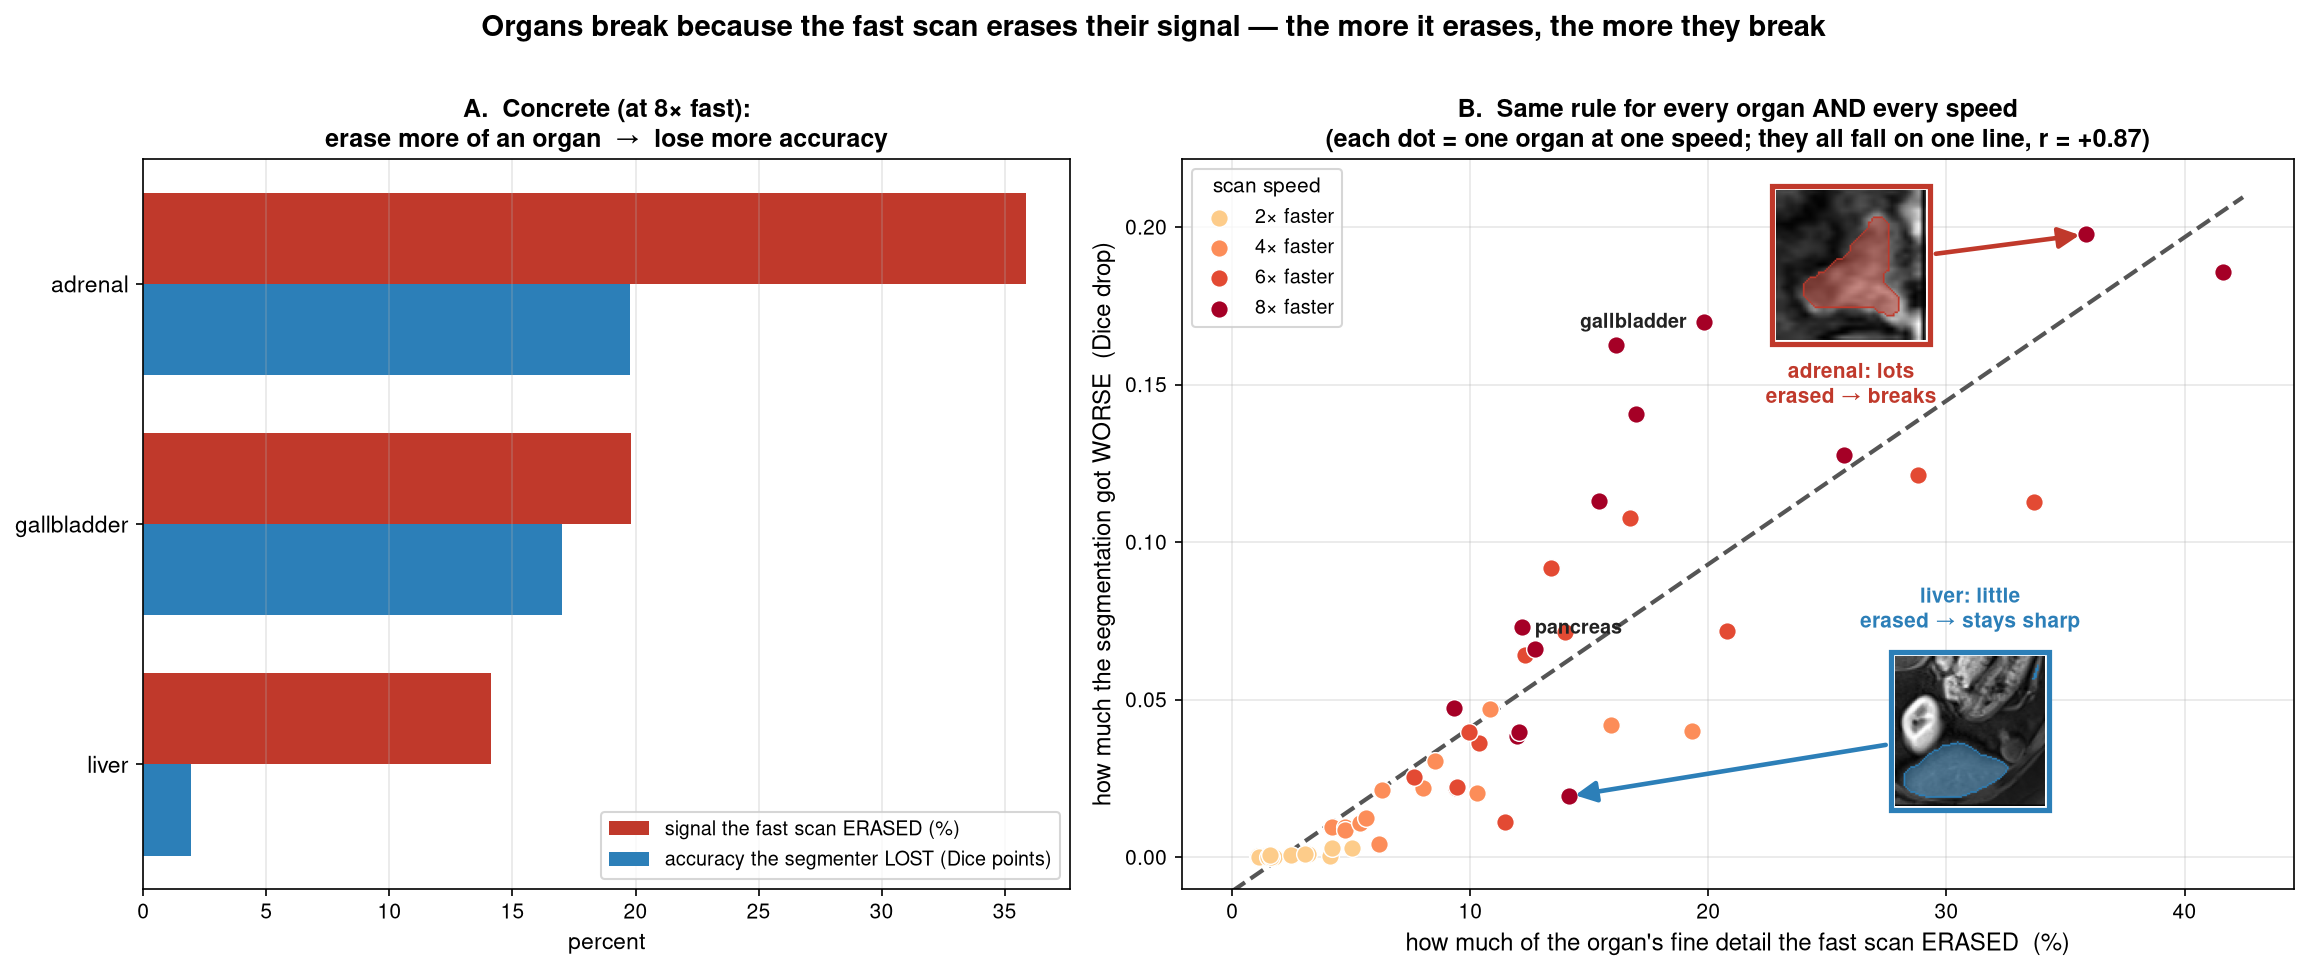
\includegraphics[width=\linewidth]{energy_causal.png}
\caption{\textbf{Removed energy predicts the task drop.} On real multicoil knee k-space, the fraction of a structure's k-space energy discarded by the undersampling mask collapses per-structure, per-rate Dice degradation onto a single relation (pooled Spearman $0.952$, Pearson $0.970$; within a fixed acceleration, $\rho=0.94$ at $R{=}6$ and $R{=}8$).}
\label{fig:energy}
\end{figure}

Why should a frequency statistic predict segmentation failure? The floor of the argument is an identity: by Parseval, the k-space energy an undersampling mask removes equals the image-domain error energy it injects. On real multicoil knee k-space \cite{desai2022skmtea} this holds at $r = 0.978 \pm 0.010$ across 44 cases, on both echoes separately ($0.976/0.987$), and within each fixed acceleration ($r = 0.77$--$0.83$) --- so it is not an artifact of the shared rate trend. On its own this is true by definition and establishes only \emph{that} acceleration hurts.

The non-tautological step is that removed energy predicts the downstream \emph{task}, not merely the image error --- and image error demonstrably does not equal task loss: reconstructions that score worse can segment better \cite{tolpadi2023}. Across six knee structures and four acceleration rates (24 structure$\times$rate points), the fraction of a structure's k-space energy removed rank-predicts its Dice degradation at pooled Spearman $0.952$ (Pearson $0.970$); crucially, \emph{within} a fixed acceleration, where the shared rate trend cannot explain it, the link persists at $\rho = 0.94$ at both $R{=}6$ and $R{=}8$ (Fig.~\ref{fig:energy}). Organs whose content sits at high radial frequency lose more of their energy budget to any variable-density mask, and the lost budget is what the segmenter misses.

\paragraph{A causal probe, reported as an informative null.}
Is the frequency \emph{location} itself causal? We tested this directly with a within-organ, energy-matched ablation: delete the same amount of energy at the organ's own spectral band versus a control band elsewhere, matching energy by varying band width at full deletion (avoiding the attenuation confound). The result is a null --- $+0.0013$ Dice difference, 95\% CI $[-0.005, +0.008]$, equivalent to zero by TOST at $p<0.0001$ --- and it is a \emph{powered} null: the design detects effects seventeen-fold smaller than the fragility phenomenon it probes. We draw the honest conclusion: the frequency signature is \emph{predictive, not causal at matched energy}. At a fixed amount of removed energy, where you remove it does not measurably matter; what matters is how much of the organ's high-frequency budget the acquisition discards. The null is thus not a gap in the story but a constraint on its interpretation --- fragility is governed by a scalar energy budget, not by an organ-specific spectral signature that a cleverer per-organ acquisition could exploit.

\section{Image-quality metrics are per-organ blind}
\label{sec:metricblind}

That aggregate reconstruction metrics decouple from downstream task performance is established prior work: Morshuis et al.\ \cite{morshuis2025} and K2S \cite{tolpadi2023} showed the aggregate decoupling on knee data, and the fastMRI challenge documented SSIM's blindness to hallucinated content \cite{muckley2021}. We do not re-claim it. Our contribution is the \emph{per-organ} resolution of that result, and it is sharper than the aggregate version: within a fixed acceleration, the standard image metric carries almost no information about \emph{which organ} is failing.

\begin{table}[t]
\centering
\caption{Image metrics are per-organ blind within a fixed acceleration (scoped to $R \ge 4$; at $R{=}2$ SSIM is near-constant and we claim nothing). Pooled across $R$, SSIM appears informative; conditioning on $R$ removes 93\% (MRISeg) / 79\% (AMOS) of the correlation. The blindness is metric-general: at $R{=}8$, neither PSNR nor SSIM predicts per-case tail-organ Dice.}
\label{tab:metricblind}
\begin{tabular}{@{}llr@{}}
\toprule
Predictor $\to$ target & Scope & $\rho$ \\
\midrule
SSIM $\to$ per-organ Dice & pooled across $R$ (MRISeg) & $0.54$ \\
SSIM $\to$ per-organ Dice & within-$R$, $R\ge4$ (MRISeg) & $0.037$ \\
SSIM $\to$ per-organ Dice & within-$R$, $R\ge4$ (AMOS) & $0.083$ \\
\midrule
PSNR $\to$ tail Dice & across cases, $R{=}8$ (MRISeg) & $-0.205$ \\
SSIM $\to$ tail Dice & across cases, $R{=}8$ (MRISeg) & $-0.093$ \\
\bottomrule
\end{tabular}
\end{table}

Table~\ref{tab:metricblind} quantifies the collapse. Pooled across acceleration factors, SSIM correlates with per-organ Dice at $\rho = 0.54$ --- but this is the shared rate trend in disguise. Conditioning on $R$ (scoped to $R \ge 4$, where SSIM actually varies) collapses the correlation to $0.037$ on MRISegmentator (a 93\% reduction) and $0.083$ on AMOS (79\%). The blindness is metric-general, not an SSIM idiosyncrasy: at $R{=}8$, across the 240 test cases, PSNR predicts tail-organ Dice at $\rho = -0.205$ and SSIM at $\rho = -0.093$ --- both approximately zero, and not for lack of variation in the metrics themselves (at $R{=}8$ PSNR spans an SD of 2.4\,dB and SSIM an SD of 0.035 across cases). A site certifying an accelerated protocol by global image quality would pass reconstructions in which the adrenal glands have already been lost.

\begin{figure}[t]
\centering
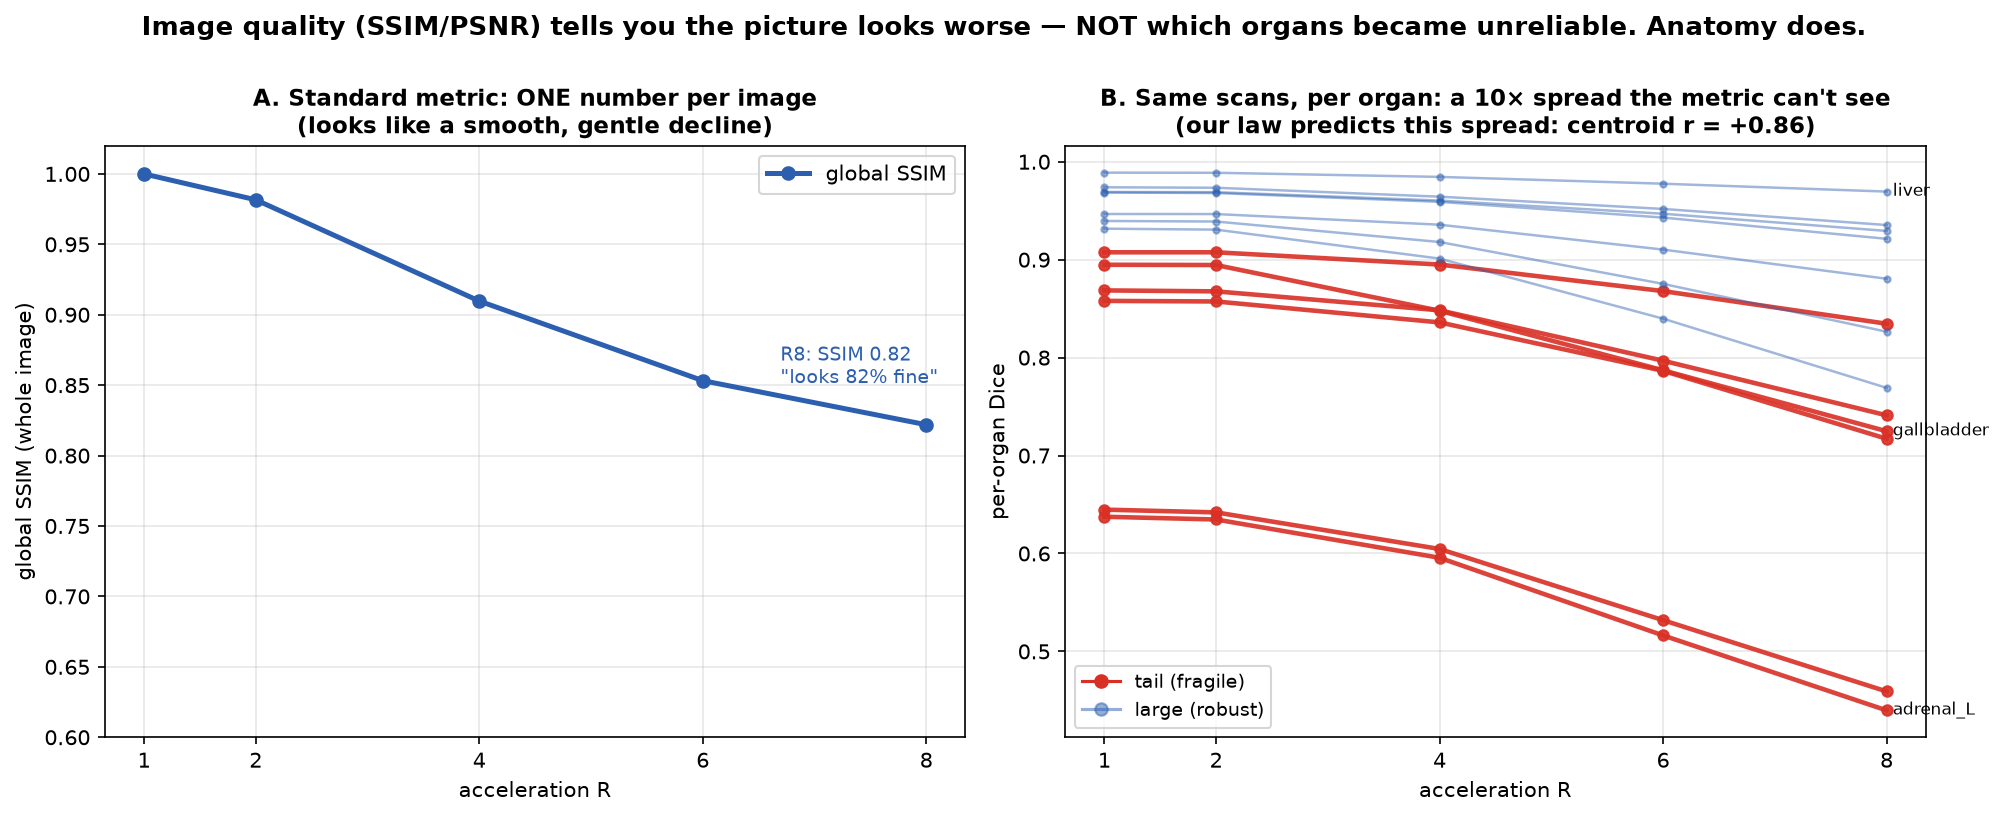
\includegraphics[width=\linewidth]{metric_vs_law.png}
\caption{\textbf{Global metrics are blind; anatomy predicts.} Predicting \emph{which} organ fails: global SSIM/PSNR operate at $\rho \approx 0$ within a fixed acceleration; an organ-local SSIM recovers some signal ($r=+0.38$) but requires the reconstructed scan; the spectral centroid predicts at $r=+0.86$ from anatomy alone, before any scan is accelerated.}
\label{fig:metricvslaw}
\end{figure}

Figure~\ref{fig:metricvslaw} makes the constructive point. The information needed to anticipate per-organ failure is simply not present in a global reconstruction metric ($\rho \approx 0$ within-$R$). An organ-localized SSIM recovers part of it ($r=+0.38$) but is post-hoc --- it requires the accelerated scan and reconstruction to already exist. The spectral centroid of Sec.~\ref{sec:law} predicts at $r=+0.86$ \emph{a priori}. For certifying accelerated protocols against downstream segmentation, per-organ anatomy is a better instrument than image fidelity.

\section{A per-organ acceleration budget}
\label{sec:budget}

Because fragility is predictable, it can be turned into an actionable, per-organ deliverable. We define an organ's \emph{acceleration budget} $R^\ast$ as the largest acceleration at which its Dice stays within a fixed tolerance of its fully sampled value,
\begin{equation}
R^\ast_{\tau}(\Omega) \;=\; \max\bigl\{\, R \;:\; \mathrm{Dice}_\Omega(R) \,\ge\, (1-\tau)\,\mathrm{Dice}_\Omega(1) \,\bigr\},
\label{eq:rstar}
\end{equation}
computed by linear interpolation over the tested rates $R\in\{1,2,4,6,8\}$ and censored at the tested maximum. Table~\ref{tab:rstar} reports the released budget at a relative tolerance of $\tau=0.10$ (10\% of the organ's $R{=}1$ Dice) on both datasets \cite{mrisegmentator2024,amos2022}. A stricter absolute tolerance of $0.05$ Dice shifts individual values downward (adrenals $R^\ast\!\approx\!4.2$ on MRISegmentator) but broadly preserves the ordering (cross-dataset $\rho{=}0.95$); at the fragile end gallbladder ($4.1$) slips below the adrenals ($4.2/4.3$); we therefore present $R^\ast$ as a robust \emph{ordering}, not a precise per-organ number.

\begin{table}[t]
\centering
\caption{Per-organ acceleration budgets $R^\ast$ (Eq.~\ref{eq:rstar}, $\tau=10\%$ relative tolerance, linear interpolation over $R\in\{1,2,4,6,8\}$). Entries ``$>8$'' are censored at the maximum tested acceleration (the released file records these as 8.5); ``---'' = organ not evaluated on AMOS. The fragile organs exhaust their budget at roughly half the acceleration the robust organs tolerate.}
\label{tab:rstar}
\small
\begin{tabular}{lcc}
\toprule
Organ & $R^\ast$ MRISeg & $R^\ast$ AMOS \\
\midrule
Adrenal L    & 4.6 & 4.3 \\
Adrenal R    & 4.7 & 3.7 \\
Gallbladder  & 5.4 & 4.4 \\
Colon        & 6.0 & --- \\
Duodenum     & 6.4 & 6.3 \\
Esophagus    & 6.5 & 6.4 \\
Small bowel  & 7.2 & --- \\
Pancreas     & $>8$ & $>8$ \\
Stomach      & $>8$ & $>8$ \\
Spleen       & $>8$ & $>8$ \\
Kidney L     & $>8$ & $>8$ \\
Kidney R     & $>8$ & $>8$ \\
Liver        & $>8$ & $>8$ \\
\bottomrule
\end{tabular}
\end{table}

\begin{figure}[t]
\centering
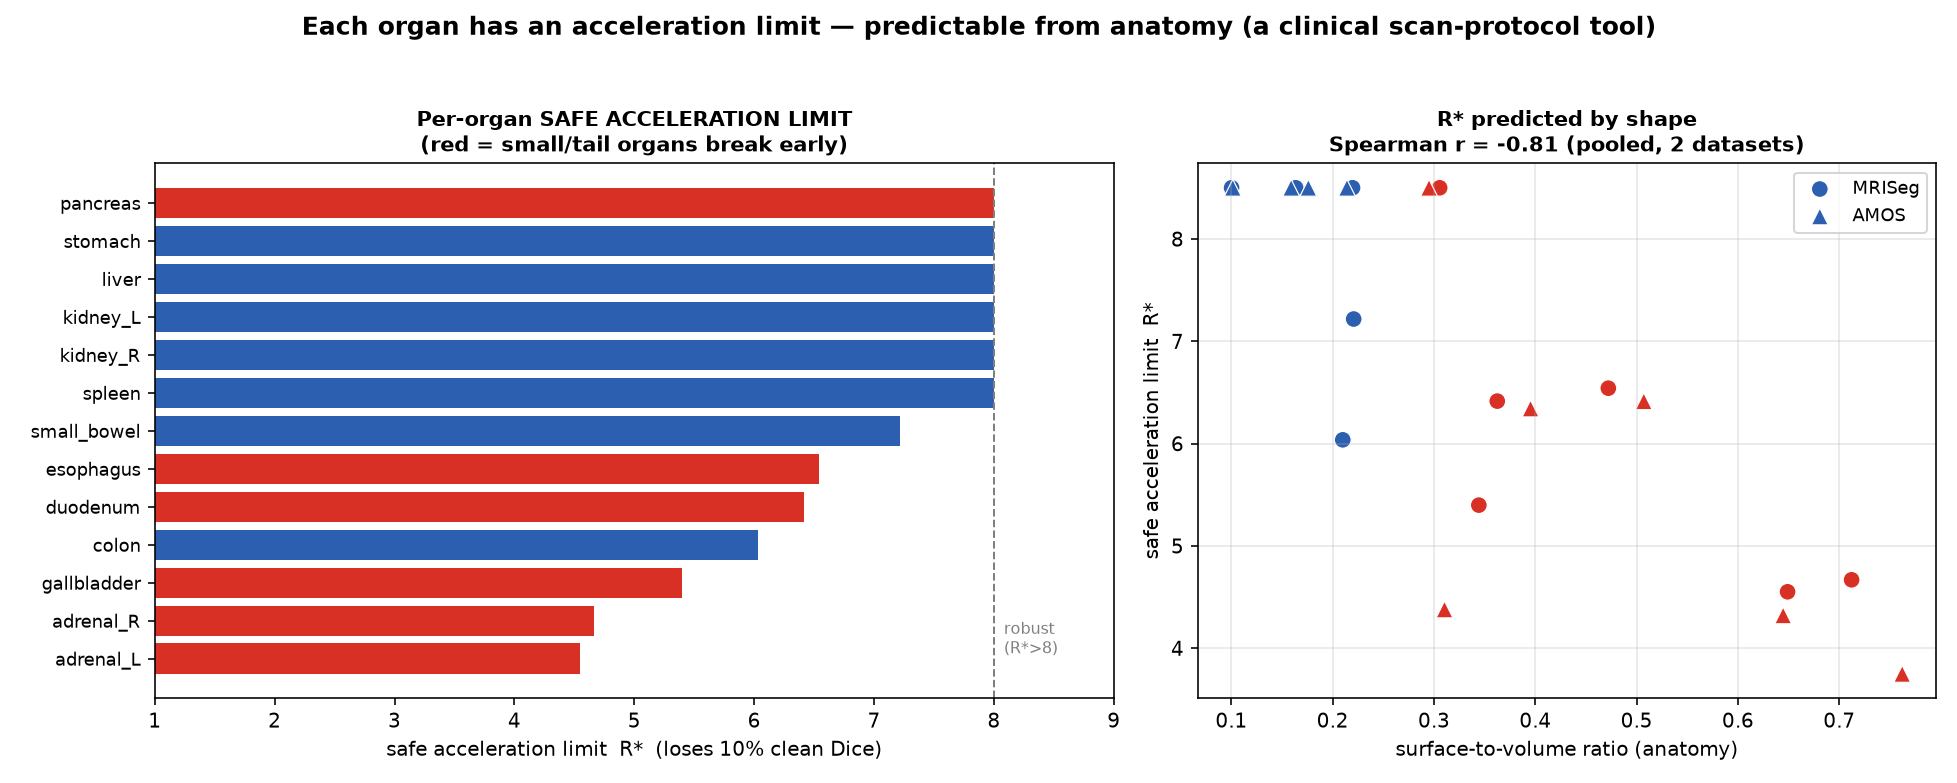
\includegraphics[width=\linewidth]{critical_R.png}
\caption{The acceleration budget. \textbf{Left:} per-organ safe limits $R^\ast$ --- the adrenal glands and gallbladder are flagged near $R\!\approx\!4$--$5$ while the solid organs stay within tolerance over the whole tested range. \textbf{Right:} the spectral centroid, computed from fully sampled anatomy alone, rank-predicts the budget (Spearman $-0.86$ MRISegmentator, $-0.91$ AMOS).}
\label{fig:rstar}
\end{figure}

The budget separates the abdomen cleanly (Fig.~\ref{fig:rstar}). The adrenal glands exhaust their budget at $R^\ast\!=\!3.7$--$4.7$ and the gallbladder at $4.4$--$5.4$; the hollow gastrointestinal structures (colon, duodenum, esophagus, small bowel) fall in an intermediate band of $R^\ast\!\approx\!6$--$7$; and the liver, kidneys, spleen, stomach, and pancreas remain within the 10\% tolerance over the entire tested range ($R^\ast>8$). The \emph{ordering} of these budgets agrees across the two datasets at Spearman $\rho=0.989$ over the eleven shared organs. Two honest caveats attach to that figure: it is inflated by ceiling ties (six of the eleven shared organs sit at the censored maximum in both datasets), and the stricter $0.05$-absolute definition gives $\rho=0.95$ --- still a near-perfect replication of the ranking, which is the claim we make.

Crucially, the budget is predictable \emph{a priori}. The spectral centroid of Sec.~4,
\begin{equation}
c_\Omega \;=\; \frac{\sum_{\mathbf{k}} \lVert \mathbf{k} \rVert \, \lvert \hat{x}_\Omega(\mathbf{k}) \rvert^{2}}{\sum_{\mathbf{k}} \lvert \hat{x}_\Omega(\mathbf{k}) \rvert^{2}},
\end{equation}
computed from the fully sampled image before any accelerated acquisition or segmenter is run, rank-predicts $R^\ast$ at Spearman $-0.86$ on MRISegmentator and $-0.91$ on AMOS, stable across five folds ($-0.85\pm0.03$). High-centroid organs have low budgets, and the mapping requires no acceleration experiment: for a new structure or dataset, an anatomy-derived fragility ordering is available before any undersampled scan is acquired.

The clinical reading is a per-organ traffic light. A site protocolizing an accelerated abdominal sequence can look up the structure of interest rather than trusting a scan-level image-quality score: at $R=6$, liver, kidney, and spleen segmentation sit comfortably inside budget, the bowel is marginal, and adrenal assessment is already outside its safe limit --- exactly the failure that the aggregate Dice and the image metrics of Sec.~6 average away. The full $R^\ast$ table and the centroid predictor are released with the paper.

\section{What fixes it --- and what does not}
\label{sec:fixes}

\subsection{Matching the training distribution: mixed-$R$}
\label{sec:mixedr}

The single intervention that reliably moves the fragile organs is not a reweighted loss or a steered reconstruction but \emph{matching the training distribution to the degradation}: training the segmenter across acceleration factors rather than at a single one (mixed-$R$; used for reconstruction in prior work \cite{yao2022,razumov2023}, here evaluated for downstream per-organ segmentation). The effect replicates on two anatomies. On real multicoil knee k-space \cite{desai2022skmtea}, mixed-$R$ training improves tail-structure Dice by $+0.134$ ($p=2\times10^{-12}$). On abdominal MRI, a mixed-$R$ nnU-Net \cite{isensee2021} deployed at $R=8$ raises mean tail-organ Dice from $0.650$ to $0.738$ ($+0.088$; Wilcoxon $p=4\times10^{-41}$), improving 239 of 240 test cases.

The per-organ pattern identifies the mechanism: mixed-$R$ \emph{helps the worst organs most}. The per-organ gain is strongly anti-correlated with the organ's baseline Dice (Spearman $\rho{=}-0.93$): the right adrenal gains $+0.146$ ($0.423\!\to\!0.569$) while the liver gains $+0.009$, a sixteen-fold spread, and the fragile-organ mean gain is $+0.090$ against $+0.043$ for the robust organs. The gain also correlates with the spectral centroid (Spearman $\rho=0.824$), but this must be read with its caveat: the partial correlation of gain with centroid, controlling for baseline Dice, is essentially zero ($-0.01$). The mechanism is therefore weakest-organ regularization under covariate shift --- mixed-$R$ rescues whichever organs are worst off --- not a centroid-specific rescue, and we state it as such.

We are equally deliberate about the magnitude. The $+0.088$ is measured against an $R2$-trained model deployed out-of-distribution at $R=8$. Against a properly matched $R8$-trained baseline the gain is a modest $+0.019$, and a plain Focal--Tversky loss slightly exceeds it there. The direction is bulletproof (239/240 cases); the value of mixed-$R$ is \emph{zero-shot deployment} --- one model that handles unseen accelerations without target-specific retraining --- rather than a large gain over a well-tuned matched baseline.

\subsection{What does not work: reweighting the loss, the reconstruction, and the sampler}
\label{sec:negatives}

Against this, every intervention that tries to \emph{emphasize} fragile content at a fixed acquisition fails, ties, or is subsumed. We report all of them.

\paragraph{Loss-side.} A fragility-weighted cross-entropy produces a real but small gain at $R=8$ ($0.650\!\to\!0.672$ tail Dice, $+0.022$) --- and is entirely subsumed by mixed-$R$: mixed-$R$ alone reaches $0.738$ ($+0.088$), and adding the fragility weighting on top of mixed-$R$ gives $0.737$, i.e.\ nothing further ($-0.001$). A fragility-weighted segmentation loss is statistically indistinguishable from uniform weighting ($p=0.77$), and a full sweep of per-organ loss weightings stays inside the seed-noise floor.

\paragraph{Reconstruction-side.} Steering a task-driven reconstruction by the fragility spectrum (FG-TDR, best boundary-weighted variant) statistically \emph{ties} mixed-$R$ ($-0.003$ Dice, $p=0.18$) --- a tie, not a win, purchased at substantially higher pipeline complexity.

\paragraph{Acquisition-side.} In a 2-D proof-of-concept at $R=8$, a LOUPE-style learned mask \cite{bahadir2020loupe,huijben2020,bakker2020} beats fixed variable-density sampling by $+0.044\pm0.025$ tail Dice across three seeds (seed-level $p=0.128$; underpowered at $n=3$, so we claim a consistent direction, not significance). But adding a fragility prior on top of the learned mask is a wash ($-0.007\pm0.004$), and the explicitly steered variant (FG-LOUPE, biasing the mask toward the fragile organs' spectra via a coverage penalty) is \emph{negative}: $-0.089$ tail Dice versus plain LOUPE. An audit found two compounding failure modes: (i) the fragility target is high-frequency-pathological --- normalizing the fragile-organ spectrum by the full-image spectrum, which decays with radial frequency, inflates the peripheral k-space lines, so the target points at the highest frequencies; and (ii) the cross-entropy coverage penalty has an unbounded gradient ($-t_k/q_k \to -\infty$ as $q_k\to 0$) that forces the mask onto the target even at small penalty weights ($\lambda=0.05$ and $0.15$ produce near-identical masks), collapsing the learned sampler into a fixed high-frequency mask that is worse than variable density. The lesson is itself a finding: task-driven learned sampling is already near-optimal, and a hand-computed frequency prior removes the low-frequency coverage every good mask needs.

\subsection{The through-line}
\label{sec:throughline}

One pattern covers every experiment in this section. Interventions that reweight --- in the segmentation loss, in the reconstruction objective, or in the sampling pattern --- fail, tie, or are subsumed, while the one intervention that changes what the model is \emph{trained on} improves 239 of 240 cases on two anatomies, one of them on real k-space. Per-organ fragility is, on this evidence, unfixable by post-hoc modeling at a fixed acquisition and scale: the deficit is information the acquisition has already discarded, and no emphasis scheme restores it. You cannot reweight your way out of deleted k-space --- match the training distribution to the degradation instead.

\section{Limitations}
\label{sec:limitations}

We state the scope conditions of this study plainly; several are themselves findings.

\paragraph{Simulated abdominal k-space.}
No public abdominal dataset pairs raw multicoil k-space with multi-organ segmentation labels, so all abdominal results use retrospective variable-density undersampling of magnitude images; only the knee results (Parseval identity, energy$\rightarrow$task link, mixed-$R$ mitigation) run on real acquired k-space~\cite{desai2022skmtea,zbontar2018fastmri}. We defend the simulation directly: replacing the magnitude-only pipeline with a full complex multicoil forward model $A = M F S$ (sampling mask, Fourier transform, coil sensitivities) preserves the per-organ fragility ordering at Spearman $\rho=0.978$. The ordering, which carries every downstream claim, is therefore not an artifact of the simplified forward model; absolute Dice values under a prospective acquisition may still differ.

\paragraph{The inferential unit is the organ.}
The fragility law is a rank correlation over $n=13$ organs (MRISegmentator~\cite{mrisegmentator2024}) and $n=11$ shared organ identities (AMOS~\cite{amos2022}) --- a small sample of non-independent units drawn from a single body region. The case-clustered bootstrap (resampling the 240 test cases) gives a 95\% CI of $[0.824, 0.879]$ around $\rho=0.863$, but this addresses case-sampling noise \emph{only}; it does not enlarge the organ-level $n$, and no resampling scheme can. The 41 whole-body TotalSegmentator structures~\cite{wasserthal2023totalseg} and the cross-dataset replication mitigate, but do not remove, this limitation.

\paragraph{The difficulty dissociation holds at full resolution only.}
On the abdomen ($n=13$) the centroid is confounded with baseline difficulty: the partial correlation of centroid with drop given clean-image Dice is $0.16$ (n.s.), so no independence claim is possible there. The dissociation we report comes from the 41 whole-body structures at full-resolution reconstruction (partial $\rho=0.389$, permutation $p=0.0067$; $\rho=0.66$, $p=0.0001$ on the 30 gradually-degrading structures; $215/296=72.6\%$ of difficulty-matched pairs ordered correctly). We disclose that under a fast off-the-shelf reconstruction preprocessing the partial collapses to $0.141$ (n.s.): the over-and-above-difficulty result is a full-resolution result.

\paragraph{Predictor identifiability on AMOS.}
On AMOS the spectral centroid is statistically inseparable from the high-frequency energy fraction: a high-frequency image-energy descriptor ties it exactly ($\rho=0.855$ for both, identical permutation $p$). The centroid leads only on MRISegmentator ($0.863$ vs.\ $0.852$ for the next-best descriptor). We therefore claim a \emph{high-frequency anatomy signature}, with the centroid as its physical representative --- not the centroid specifically.

\paragraph{The law is an abdominal multi-organ result.}
On knee tissues (SKM-TEA~\cite{desai2022skmtea}) the centroid$\rightarrow$drop ordering \emph{reverses sign}. We report this as the law's falsification boundary and state it as a scope condition: the knee offers a narrow centroid range across few, spectrally similar tissues, where the monotone relationship degrades to noise. The law should not be extrapolated beyond multi-organ abdominal (and, with the stated caveats, whole-body) settings without re-validation.

\paragraph{AMOS is consistently weaker.}
Every effect is smaller on AMOS than on MRISegmentator: the law ($0.855$ vs.\ $0.863$), the within-$R$ metric-blindness collapse ($79\%$ vs.\ $93\%$), and predictor identifiability (above). We report both datasets throughout rather than the more favorable one.

\paragraph{Sampling experiments are a 2D zero-filled proof of concept.}
The learned-sampling experiments (B1) use LOUPE-style masks~\cite{bahadir2020loupe} with 2D zero-filled reconstruction, not a learned reconstruction or 3D acquisition. Learned masks beat fixed variable-density sampling by $+0.044 \pm 0.025$ Dice across seeds, but the seed-level test is underpowered ($p=0.128$ at $n=3$ seeds). Adding a fragility prior on top is a wash ($-0.007 \pm 0.004$), and the steered FG-LOUPE variant is negative ($-0.089$, with two audited failure modes). We report these as honest negatives consistent with the shared-budget account, not as evidence that task-driven sampling~\cite{razumov2023,huijben2020,weiss2021} cannot work in stronger pipelines.

\paragraph{Single architecture family.}
All segmentation results use the nnU-Net family~\cite{isensee2021}. nnU-Net is the standard and strongest baseline for this setting, but the per-organ fragility magnitudes --- and the finding that mitigation is unavailable by post-hoc modeling at fixed acquisition and scale --- are established for this architecture family and our training scale, not universally.

\section{Conclusion}
\label{sec:conclusion}

Under k-space acceleration, multi-organ abdominal segmentation does not degrade uniformly: per-organ Dice loss spans an order of magnitude (adrenal $-0.198$ vs.\ liver $-0.019$; 13/13 organs significant after Holm correction, replicated on a second dataset), and a single aggregate Dice number hides all of it. This failure is predictable \emph{before any accelerated scan or segmenter is run}: a high-frequency anatomy signature --- the spectral centroid as its physical representative --- rank-predicts the drop at $\rho \approx 0.86$ on both datasets. The mechanism is grounded in real k-space: the energy an undersampling mask removes rank-predicts the downstream Dice degradation at $0.952$ pooled and $0.94$ within fixed acceleration --- a task link that escapes the Parseval tautology, since image error and task loss are known to decouple~\cite{tolpadi2023,morshuis2025}.

Three practical consequences follow. First, the per-organ acceleration budget $R^{*}$ --- unsafe beyond $R\approx4$ for the adrenals, $R=8$ and above for liver and kidneys --- is computable a priori and its ordering agrees across datasets ($\rho=0.989$); accelerated protocols should be certified per target organ, not per image. Second, image-quality metrics are within-acceleration blind to per-organ task failure at $R\geq4$ (PSNR$\rightarrow$tail-Dice $\rho=-0.205$, SSIM $\rho=-0.093$ at $R{=}8$), extending the aggregate metric--task decoupling established by prior work~\cite{morshuis2025,tolpadi2023,muckley2021} to per-organ resolution: evaluation of accelerated MRI for downstream use should report per-organ task metrics. Third, the deficit is unfixable by post-hoc modeling at fixed acquisition and scale: fragility-guided reconstruction ties mixed-$R$ training at best ($-0.003$, $p=0.18$), fragility-weighted losses are indistinguishable from uniform ($p=0.77$), a full weighting sweep stays inside seed noise. The one intervention that moves the needle is matching the training distribution to the degradation --- mixed-acceleration training, directionally unambiguous at 239/240 cases ($p=4\times10^{-41}$) though modest against a matched same-$R$ baseline ($+0.019$) --- and it acts as weakest-organ regularization: the gain anti-correlates with baseline Dice at Spearman $\rho{=}-0.93$, helping the worst organs most.

The through-line is a single scalar: how much of an organ's high-frequency energy budget the acquisition discards. That scalar is set at acquisition time, which is why no reweighting --- in the reconstruction, the loss, or the sampling pattern --- recovers it, and why the constructive deliverables of this paper are the ones computable before acquisition: the fragility predictor and the per-organ acceleration budget.

\section*{Reproducibility and release}

All code, the per-organ acceleration-budget tables ($R^{*}$ for both datasets), the spectral-centroid predictor implementation, the undersampling-mask generator (per-case deterministic seeds), and the serialized per-experiment result files backing every number in this paper are released at \url{https://github.com/AlfinPutra23/MRI_Fragility}. All datasets used are public: MRISegmentator-Abdomen~\cite{mrisegmentator2024}, AMOS~\cite{amos2022}, SKM-TEA~\cite{desai2022skmtea}, and fastMRI~\cite{zbontar2018fastmri}; segmentation uses the public nnU-Net framework~\cite{isensee2021}. Every reported statistic, including the negative results, can be regenerated from the released artifacts without retraining.

\begin{thebibliography}{30}

\bibitem{akcakaya2022}
M.~Ak\c{c}akaya, B.~Yaman, H.~Chung, and J.~C. Ye.
\newblock Unsupervised deep learning methods for biological image reconstruction and enhancement: An overview from a signal processing perspective.
\newblock {\em IEEE Signal Processing Magazine}, 39(2):28--44, 2022.

\bibitem{bahadir2020loupe}
C.~D. Bahadir, A.~Q. Wang, A.~V. Dalca, and M.~R. Sabuncu.
\newblock Deep-learning-based optimization of the under-sampling pattern in {MRI}.
\newblock {\em IEEE Transactions on Computational Imaging}, 6:1139--1152, 2020.

\bibitem{bakker2020}
T.~Bakker, H.~van Hoof, and M.~Welling.
\newblock Experimental design for {MRI} by greedy policy search.
\newblock In {\em Advances in Neural Information Processing Systems (NeurIPS)}, 2020.

\bibitem{chaudhari2020}
A.~S. Chaudhari, C.~M. Sandino, E.~K. Cole, D.~B. Larson, G.~E. Gold, S.~S. Vasanawala, M.~P. Lungren, B.~A. Hargreaves, and C.~P. Langlotz.
\newblock Prospective deployment of deep learning in {MRI}: A framework for important considerations, challenges, and recommendations for best practices.
\newblock {\em Journal of Magnetic Resonance Imaging}, 54(2):357--371, 2021.

\bibitem{defazio2020}
A.~Defazio, T.~Murrell, and M.~P. Recht.
\newblock {MRI} banding removal via adversarial training.
\newblock In {\em Advances in Neural Information Processing Systems (NeurIPS)}, 2020.

\bibitem{desai2022skmtea}
A.~D. Desai, A.~M. Schmidt, E.~B. Rubin, C.~M. Sandino, M.~S. Black, V.~Mazzoli, K.~J. Stevens, R.~Boutin, C.~R\'{e}, G.~E. Gold, B.~A. Hargreaves, and A.~S. Chaudhari.
\newblock {SKM-TEA}: A dataset for accelerated {MRI} reconstruction with dense image labels for quantitative clinical evaluation.
\newblock In {\em Advances in Neural Information Processing Systems (NeurIPS) Datasets and Benchmarks Track}, 2021.

\bibitem{hammernik2018}
K.~Hammernik, T.~Klatzer, E.~Kobler, M.~P. Recht, D.~K. Sodickson, T.~Pock, and F.~Knoll.
\newblock Learning a variational network for reconstruction of accelerated {MRI} data.
\newblock {\em Magnetic Resonance in Medicine}, 79(6):3055--3071, 2018.

\bibitem{heckel2024}
R.~Heckel, M.~Jacob, A.~Chaudhari, O.~Perlman, and E.~Shimron.
\newblock Deep learning for accelerated and robust {MRI} reconstruction.
\newblock {\em Magnetic Resonance Materials in Physics, Biology and Medicine}, 37:335--368, 2024.

\bibitem{huijben2020}
I.~A.~M. Huijben, B.~S. Veeling, and R.~J.~G. van Sloun.
\newblock Deep probabilistic subsampling for task-adaptive compressed sensing.
\newblock In {\em International Conference on Learning Representations (ICLR)}, 2020.

\bibitem{isensee2021}
F.~Isensee, P.~F. Jaeger, S.~A.~A. Kohl, J.~Petersen, and K.~H. Maier-Hein.
\newblock {nnU-Net}: A self-configuring method for deep learning-based biomedical image segmentation.
\newblock {\em Nature Methods}, 18(2):203--211, 2021.

\bibitem{amos2022}
Y.~Ji, H.~Bai, C.~Ge, J.~Yang, Y.~Zhu, R.~Zhang, Z.~Li, L.~Zhang, W.~Ma, X.~Wan, and P.~Luo.
\newblock {AMOS}: A large-scale abdominal multi-organ benchmark for versatile medical image segmentation.
\newblock In {\em Advances in Neural Information Processing Systems (NeurIPS) Datasets and Benchmarks Track}, 2022.

\bibitem{knoll2020}
F.~Knoll, T.~Murrell, A.~Sriram, N.~Yakubova, J.~Zbontar, M.~Rabbat, A.~Defazio, M.~J. Muckley, D.~K. Sodickson, C.~L. Zitnick, and M.~P. Recht.
\newblock Advancing machine learning for {MR} image reconstruction with an open competition: Overview of the 2019 {fastMRI} challenge.
\newblock {\em Magnetic Resonance in Medicine}, 84(6):3054--3070, 2020.

\bibitem{lustig2007}
M.~Lustig, D.~Donoho, and J.~M. Pauly.
\newblock Sparse {MRI}: The application of compressed sensing for rapid {MR} imaging.
\newblock {\em Magnetic Resonance in Medicine}, 58(6):1182--1195, 2007.

\bibitem{morshuis2025}
J.~N. Morshuis, et~al.
\newblock Segmentation performance under undersampled {MRI} reconstruction.
\newblock {\em arXiv preprint arXiv:2508.18975}, 2025.

\bibitem{muckley2021}
M.~J. Muckley, B.~Riemenschneider, A.~Radmanesh, S.~Kim, G.~Jeong, J.~Ko, Y.~Jun, H.~Shin, D.~Hwang, M.~Mostapha, et~al.
\newblock Results of the 2020 {fastMRI} challenge for machine learning {MR} image reconstruction.
\newblock {\em IEEE Transactions on Medical Imaging}, 40(9):2306--2317, 2021.

\bibitem{pineda2020}
L.~Pineda, S.~Basu, A.~Romero, R.~Calandra, and M.~Drozdzal.
\newblock Active {MR} k-space sampling with reinforcement learning.
\newblock In {\em Medical Image Computing and Computer Assisted Intervention (MICCAI)}, 2020.

\bibitem{radmanesh2022}
A.~Radmanesh, M.~J. Muckley, T.~Murrell, E.~Lindsey, A.~Sriram, F.~Knoll, D.~K. Sodickson, and Y.~W. Lui.
\newblock Exploring the acceleration limits of deep learning variational network--based two-dimensional brain {MRI}.
\newblock {\em Radiology: Artificial Intelligence}, 4(6):e210313, 2022.

\bibitem{rahaman2019}
N.~Rahaman, A.~Baratin, D.~Arpit, F.~Draxler, M.~Lin, F.~Hamprecht, Y.~Bengio, and A.~Courville.
\newblock On the spectral bias of neural networks.
\newblock In {\em International Conference on Machine Learning (ICML)}, pages 5301--5310, 2019.

\bibitem{razumov2023}
A.~Razumov, O.~Y. Rogov, and D.~V. Dylov.
\newblock Optimal {MRI} undersampling patterns for ultimate benefit of medical vision tasks.
\newblock {\em Magnetic Resonance Imaging}, 103:37--47, 2023.

\bibitem{rotkopf2026}
L.~T. Rotkopf, et~al.
\newblock Breast {MRI} segmentation under k-space undersampling.
\newblock Preprint, 2026.

\bibitem{sanchez2020}
T.~Sanchez, B.~G\"{o}zc\"{u}, R.~B. van Heeswijk, A.~Eftekhari, E.~Il{\i}cak, T.~\c{C}ukur, and V.~Cevher.
\newblock Scalable learning-based sampling optimization for compressive dynamic {MRI}.
\newblock In {\em IEEE International Conference on Acoustics, Speech and Signal Processing (ICASSP)}, pages 8584--8588, 2020.

\bibitem{sriram2020}
A.~Sriram, J.~Zbontar, T.~Murrell, A.~Defazio, C.~L. Zitnick, N.~Yakubova, F.~Knoll, and P.~Johnson.
\newblock End-to-end variational networks for accelerated {MRI} reconstruction.
\newblock In {\em Medical Image Computing and Computer Assisted Intervention (MICCAI)}, pages 64--73, 2020.

\bibitem{tolpadi2023}
A.~A. Tolpadi, U.~Bharadwaj, K.~T. Gao, R.~Bhattacharjee, F.~G. Gassert, J.~Luitjens, et~al.
\newblock {K2S} challenge: From undersampled k-space to automatic segmentation.
\newblock {\em Bioengineering}, 10(2):267, 2023.

\bibitem{wasserthal2023totalseg}
J.~Wasserthal, H.-C. Breit, M.~T. Meyer, M.~Pradella, D.~Hinck, A.~W. Sauter, T.~Heye, D.~T. Boll, J.~Cyriac, S.~Yang, M.~Bach, and M.~Segeroth.
\newblock {TotalSegmentator}: Robust segmentation of 104 anatomic structures in {CT} images.
\newblock {\em Radiology: Artificial Intelligence}, 5(5):e230024, 2023.

\bibitem{weiss2021}
T.~Weiss, O.~Senouf, S.~Vedula, O.~Michailovich, M.~Zibulevsky, and A.~Bronstein.
\newblock {PILOT}: Physics-informed learned optimized trajectories for accelerated {MRI}.
\newblock {\em Machine Learning for Biomedical Imaging (MELBA)}, 1:1--23, 2021.

\bibitem{xu2019}
Z.-Q.~J. Xu, Y.~Zhang, T.~Luo, Y.~Xiao, and Z.~Ma.
\newblock Frequency principle: {Fourier} analysis sheds light on deep neural networks.
\newblock {\em arXiv preprint arXiv:1901.06523}, 2019.

\bibitem{yao2022}
J.~Yao and M.~S. Hansen.
\newblock Deep learning {MRI} reconstruction trained across acceleration factors.
\newblock Preprint, 2022.

\bibitem{yin2019}
D.~Yin, R.~Gontijo~Lopes, J.~Shlens, E.~D. Cubuk, and J.~Gilmer.
\newblock A {Fourier} perspective on model robustness in computer vision.
\newblock In {\em Advances in Neural Information Processing Systems (NeurIPS)}, 2019.

\bibitem{zbontar2018fastmri}
J.~Zbontar, F.~Knoll, A.~Sriram, T.~Murrell, Z.~Huang, M.~J. Muckley, A.~Defazio, R.~Stern, P.~Johnson, M.~Bruno, et~al.
\newblock {fastMRI}: An open dataset and benchmarks for accelerated {MRI}.
\newblock {\em arXiv preprint arXiv:1811.08839}, 2018.

\bibitem{mrisegmentator2024}
Y.~Zhuang, T.~S. Mathai, P.~Mukherjee, B.~Khoury, B.~Kim, B.~Hou, N.~Rabbee, and R.~M. Summers.
\newblock {MRISegmentator-Abdomen}: A fully automated multi-organ and structure segmentation tool for {T1}-weighted abdominal {MRI}.
\newblock {\em arXiv preprint arXiv:2405.05944}, 2024.

\end{thebibliography}

\end{document}
